\documentclass{article}

\usepackage{geometry}
\usepackage{amsmath}
\usepackage{graphicx, eso-pic}
\usepackage{listings}
\usepackage{hyperref}
\usepackage{multicol}
\usepackage{fancyhdr}
\pagestyle{fancy}
\fancyhf{}
\hypersetup{ colorlinks=true, linkcolor=black, filecolor=magenta, urlcolor=cyan}
\geometry{ a4paper, total={170mm,257mm}, top=40mm, right=20mm, bottom=20mm, left=20mm}
\setlength{\parindent}{0pt}
\setlength{\parskip}{0.5em}
\renewcommand{\headrulewidth}{0pt}
\AddToShipoutPictureBG{%
  \AtPageUpperLeft{%
    \raisebox{-\height}{
\includegraphics[width=\paperwidth, height=30mm]{../headerarkav.png}}
  }
}
\rfoot{\thepage}
\lfoot{Competitive Programming - Arkavidia 8.0}
\lstset{
    basicstyle=\ttfamily\small,
    columns=fixed,
    extendedchars=true,
    breaklines=true,
    tabsize=2,
    prebreak=\raisebox{0ex}[0ex][0ex]{\ensuremath{\hookleftarrow}},
    frame=none,
    showtabs=false,
    showspaces=false,
    showstringspaces=false,
    prebreak={},
    keywordstyle=\color[rgb]{0.627,0.126,0.941},
    commentstyle=\color[rgb]{0.133,0.545,0.133},
    stringstyle=\color[rgb]{01,0,0},
    captionpos=t,
    escapeinside={(\%}{\%)}
}

\begin{document}

\begin{center}
    \section*{B. Banjir Kontigu} % ganti judul soal

    \begin{tabular}{ | c c | }
        \hline
        Batas Waktu  & 3s \\    % jangan lupa ganti time limit
        Batas Memori & 512MB \\  % jangan lupa ganti memory limit
        \hline
    \end{tabular}
\end{center}

\subsection*{Deskripsi}
Di Kota Arkanesia, terdapat $N$ rumah yang dinomori dengan bilangan bulat $1$ sampai $N$. Terdapat juga $M$ jalan dua arah, masing-masing menghubungkan dua rumah. Jalan ke-$i$ menghubungkan rumah bernomor $U_i$ dan $V_i$. Setiap rumah ditinggali tepat satu orang.

Arkanesia merupakan kota yang sering dilanda banjir. Uniknya, masing-masing peristiwa banjir di Arkanesia dapat dideskripsikan dengan dua bilangan bulat, misalkan $L$ dan $R$, yang menyatakan bahwa rumah bernomor $i$ terkena banjir jika dan hanya jika $L \leq i \leq R$. Untuk menangani banjir, masing-masing penghuni rumah yang terkena banjir harus melakukan salah satu dari dua aksi berikut.
\begin{enumerate}
    \item Menyalakan sistem anti banjir
    
    Penghuni rumah bernomor $i$ harus membayar biaya sebesar $A_i$ untuk menyalakan sistem anti banjir rumahnya. Setelah dinyalakan, sistem anti banjir akan aktif selama \textbf{satu} peristiwa banjir.
    \item Mengungsi ke rumah lain yang tidak terkena banjir
    
    Penghuni rumah bernomor $i$ dapat mengungsi ke rumah bernomor $j$ jika dan hanya jika terdapat sekumpulan jalan yang menghubungkan rumah bernomor $i$ dengan rumah bernomor $j$ dan rumah bernomor $j$ tidak terkena banjir (rumah dengan sistem anti banjir aktif dianggap tidak terkena banjir). Aksi ini tidak memerlukan biaya. Setiap rumah dapat menampung $10^{100}$ pengungsi.
\end{enumerate}

Arvy, seorang meteorolog Arkanesia, telah mensimulasikan $Q$ buah kejadian, masing-masing berjenis salah satu dari dua jenis berikut.
\begin{enumerate}
    \item \verb|1 i X|
    
    Biaya menyalakan sistem anti banjir rumah bernomor $i$, yaitu $A_i$, diganti menjadi $X$.
    \item \verb|2 L R|
    
    Terjadi banjir yang dideskripsikan dengan bilangan bulat $L$ dan $R$.
\end{enumerate}

Untuk setiap kejadian jenis kedua, Arvy mencatat biaya total \textbf{minimum} yang dapat dikeluarkan. Bantulah dia mencocokkan hasilnya!

\subsection*{Format Masukan}
Baris pertama masukan berisi tiga bilangan bulat: $N$, $M$, dan $Q$ $(1 \leq N, Q \leq 10^5, 0 \leq M \leq min(\frac{N(N-1)}{2}, 10^5))$ yang menyatakan banyak rumah, banyak jalan, dan banyak kejadian.

Baris kedua masukan berisi $N$ bilangan bulat $A_1, A_2, ..., A_N$ $(1 \leq A_i \leq 10^9)$ yang menyatakan biaya menyalakan sistem anti banjir masing-masing rumah sebelum kejadian pertama.

Masukan dilanjutkan dengan $M$ baris. Baris ke-$i$ berisi dua bilangan bulat $U_i$ dan $V_i$ $(1 \leq U_i, V_i \leq N, U_i \neq V_i)$ yang menyatakan bahwa terdapat jalan dua arah yang menghubungkan rumah bernomor $U_i$ dan $V_i$. Tidak ada sepasang jalan yang menghubungkan pasangan rumah yang sama.

Masukan dilanjutkan dengan $Q$ baris berisi deskripsi kejadian-kejadian. Setiap baris diawali dengan \verb|1| atau \verb|2|.
\begin{itemize}
    \item Apabila baris diawali dengan \verb|1|, masukan dilanjutkan dengan dua bilangan bulat $i$ dan $X$ $(1 \leq i \leq N, 1 \leq X \leq 10^9)$ yang menyatakan bahwa biaya menyalakan sistem anti banjir rumah bernomor $i$ diganti menjadi $X$.
    \item Apabila baris diawali dengan \verb|2|, masukan dilanjutkan dengan dua bilangan bulat $L$ dan $R$ $(1 \leq L \leq R \leq N)$ yang mendeskripsikan banjir.
\end{itemize}
Dijamin bahwa terdapat setidaknya satu baris yang diawali \verb|2|.

\subsection*{Format Keluaran}
Untuk setiap kejadian yang diawali \verb|2| (kejadian jenis kedua), keluarkan sebuah baris berisi bilangan bulat yang menyatakan total biaya minimum yang dapat dikeluarkan pada kejadian tersebut.

\begin{multicols}{2}
\subsection*{Contoh Masukan}
\begin{lstlisting}
8 6 5
8 7 6 5 4 3 2 1
3 4
6 4
3 7
8 5
6 3
1 8
2 3 4
2 1 7
1 7 7
2 1 7
2 1 2
\end{lstlisting}
\null
\columnbreak

\subsection*{Contoh Keluaran}
\begin{lstlisting}
0
9
10
7
\end{lstlisting}
\vfill
\null
\end{multicols}

\subsection*{Penjelasan}
Pada contoh masukan, Kota Arkanesia dapat digambarkan seperti berikut.

\begin{center}
    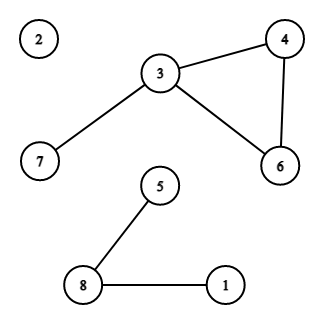
\includegraphics[scale=0.4]{sample-graph.png}    
\end{center}

Pada kejadian banjir pertama (dengan $L=3$ dan $R=4$), penghuni rumah bernomor $3$ dan $4$ dapat mengungsi ke rumah bernomor $6$, sehingga tidak ada biaya yang dikeluarkan.

Pada kejadian banjir kedua (dengan $L=1$ dan $R=7$), aksi-aksi berikut dapat dilakukan untuk mendapatkan total biaya $9$.
\begin{itemize}
    \item Penghuni rumah bernomor $2$ dan $7$ menyalakan sistem anti banjir rumahnya dengan total biaya $A_2+A_7 = 7+2 = 9$.
    \item Penghuni rumah bernomor $1$ dan $5$ mengungsi ke rumah bernomor $8$.
    \item Penghuni rumah bernomor $3$, $4$, dan $6$ mengungsi ke rumah bernomor $7$.
\end{itemize}
Dapat ditunjukkan bahwa tidak ada kumpulan aksi dengan total biaya kurang dari $9$.

\end{document}